\begin{frame}
    \frametitle{Amputation prostheses}
    \alt<1>{
    \begin{itemize}
        \item Stump prostheses
        \item Load borne by soft tissue
    \end{itemize}
        \begin{columns}
            \begin{column}{0.5\textwidth}
                \includegraphics[height=4cm]{figures/stump.png}
            \end{column}
            \begin{column}{0.5\textwidth}
                \includegraphics[height=4cm]{figures/stump-prosthesis.png}
                
                {\tiny Adapted from photo by ShotPot via \href{https://www.pexels.com/photo/man-with-prosthetic-leg-walking-by-swimming-pool-4045098/}{Pexels}}
            \end{column}
        \end{columns}
        }{}
    \alt<2>{
        \begin{itemize}
            \item Skin damage
            \item Patients may not want to wear their prostheses
        \end{itemize}
        \includegraphics[width=0.5\textwidth]{figures/stump-damage.png}

        {\tiny Adapted from \footcite{MeulenbeltHenkEJ2011SPot} }
    }{}
    

\end{frame}

\begin{frame}
    \frametitle{ITAP}
    Intraosseous Transcutaneous Amputation Prosthesis
\begin{itemize}
    \item Bone-anchored, skin crossing prosthesis
    \item Bypass the role of soft tissue
\end{itemize}
        \includegraphics[height=4.5cm]{figures/ITAP-old.jpg}
        \includegraphics[height=4.5cm]{figures/ITAP-xray.jpg}
        {\tiny \incfig[0.3]{ITAP-scheme}}

        {\tiny Adapted with permission from \footcite{Fitzpatrick2011ITAP} and \footcite{KANG20101130} }

\end{frame}

\begin{frame}
    \frametitle{ITAP}

    \includegraphics[width=1\textwidth]{figures/itap-prosthesis.jpg}

    {\tiny From \footcite{KANG20101130}}

\end{frame}

\begin{frame}
    \frametitle{What now?}

    \begin{figure}[h]\centering
    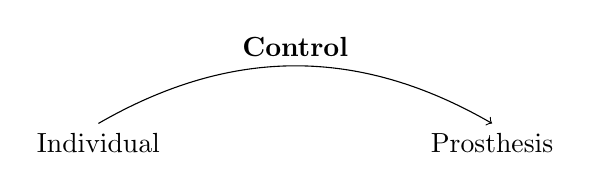
\begin{tikzpicture}
        \draw (0,0) node[below]{Individual} (5,0) node[below]{Prosthesis};
        \pause \draw[->] (0,0) to[bend left] node[midway,above]{\textbf{Control}} (5,0);
        % \draw[->] (5,-0.6) to[bend left] node[midway,below] {Feedback} (0,-0.6);
    \end{tikzpicture}
    \end{figure}
    \begin{itemize}
        \item <2-> Take advantage of ITAP
        \item <2-> Reliable control of the prosthetic
    \end{itemize}
\end{frame}